\documentclass{article}
\usepackage{graphicx} % for inserting images

% for setting up figures
\usepackage{subfigure}
\usepackage{multirow}
\usepackage{booktabs}

% set up the margins
\usepackage[margin=1.2in, inner=1.2in]{geometry}
\geometry{top=1in}

% for math stuff
% package for math stuff
\usepackage{algorithmic}
\usepackage{algorithm}
\usepackage{mathtools}
\usepackage{amssymb}
\usepackage{amsmath}

% for captions
\usepackage{caption}
%\captionsetup[figure]{font=small}
%\usepackage{subcaption}

% set up the packages for the references
\usepackage[style=science]{biblatex}
\addbibresource{refs.bib}

% set up the title
\title{Monitoring Committee Report: \\
\large Decadal climate forecasting for the energy-sector}
\author{Ben Hutchins}
\date{June 2023}

% set up the document
\begin{document}

% make the title
\maketitle

% give some background to the project in the introduction
\section*{Introduction}

As power systems transition towards a greater share of renewable energy sources, such as wind and solar PV, energy systems become increasingly vulnerable to climate variability \parencite{bloomfield2016quantifying}. As a result, there is need for longer range climate forecasting, such as seasonal and decadal forecasts, to inform both the operation and development of these changing power systems. Currently, seasonal forecasts are used to inform management decisions ahead of challenging periods for supply security, such as the winter period \parencite{national_grid_winter_2022}. However, (as far as we know) there is currently no operational usage of decadal (1-10 year) climate forecasts. Decadal forecasts seek to make predictions of the evolution of large-scale climate features over 1-10 years, a key timescale for power system planning and operation. These forecasts could be used, for example, to develop early warning systems for low-wind years, such as the those experienced in Europe during 2021 \parencite{copernicus_climate_change_service_c3s_european_2022}.\\

In order for these decadal forecasts to have value, however, they must show skill. As decadal forecasts quickly lose their predictable signal from initialization, these forecasts are often very noisy \parencite{eade2014seasonal}. As a result, large multi-model ensembles are used to extract the predictable signal in decadal forecasts. However, the models often show underconfidence, where they underestimate the predictability of the real world \parencite{eade2014seasonal}. Despite this, recent techniques outlined in \cite{smith2020north}, such as lagged ensembles and NAO-matching, have improved the skill of decadal forecasts of large modes of variability, such as the NAO and AMV.\\

As research has demonstrated the value of seasonal forecasts for the european energy-sector \parencite{clark2017skilful,thornton2019skilful}, there is potential for decadal forecasts to provide value at longer timescales, particularly with the recent findings of surprising skill in decadal NAO forecasts \parencite{smith2020north}.


% updated literature review, giving background to the specific direction //
% in which I am heading
\section*{Literature Review}

Predictability on decadal timescales derives from slowly varying, often large-scale, modes of variability; such as the El Niño-Southern Oscilation (ENSO) or the Atlantic Multidecadal variability (AMV) \parencite{smith2012current}. Decadal forecasts aim to predict changes in climate and the frequency of extremes by resolving the evolution of these drivers on timescales of 1-10 years \parencite{eade2012forecasting}. The temporal variability in these forecasts can be divided into two components; the predictable component tied to predictable modes of variability (the signal) and the unpredictable component resulting from the chaotic nature of the atmosphere (the noise) \parencite{eade2014seasonal}. Uncertainty in decadal forecasts therefore depends on the size of the predictable signal relative to the unpredictable noise (signal-to-noise ratio), among other factors. As a result, large ensembles are used to assess and quantify the uncertainty in these forecasts. \\

At seasonal and decadal timescales, numerous experiments have demonstrated the low strength of predictable signals in climate models and the unexpected high correlation with observations (given small signal-to-noise ratios) \parencite{eade2014seasonal,riddle2013cfsv2,scaife2014skillful,kang2014prediction,dunstone2016skilful,smith2020north,marcheggiani2023decadal}. This is known as the signal-to-noise paradox, which occurs when ensemble predictions from climate models show higher correlation with obsevations than their individual ensemble members \parencite{scaife2018signal}.Hence, the predictable component in models is smaller than in reality, when looking at modes of variability such as the NAO \parencite{smith2020north,dunstone2016skilful}, AO \parencite{riddle2013cfsv2,kang2014prediction} and the eddy-driven jet \parencite{marcheggiani2023decadal}.\\

Large multi-model ensembles were used to create decadal hindcasts of the NAO and AMV in \cite{smith2020north}. The moderate skill in the raw ensemble output was amplified using two techniques; increasing the ensemble size by lagging the forecasts (and adjusting the variance) and by subselecting members which have the required magnitude of NAO (NAO-matching) \parencite{smith2020north}. This demonstrated that decadal forecast skill in the North Atlantic could be amplified by reducing the noise (by lagging the ensemble) or increasing the predictable signal (through NAO-matching). However, recent results from \cite{marcheggiani2023decadal} have show that this skill may be sensitive to the period over which it is assessed; which statistically significant reductions in skill for the NAO index when assessed over the longer period from 1960-2012 insted of the shorter period from 1960-2005. They propose that this drop in skill can be explained by the DCPP-A models failing to capture a return to positive NAO indexes associated with a stronger and warmer jet as well as also failing to capture recent cooling of the subpolar North Atlantic \parencite{marcheggiani2023decadal}.\\


In order to provide value to the energy-sector from decadal forecasts, the skill in large-scale phenomena must be translated into skill for relevant surface variables, such as surface temperature, wind speeds and incoming solar radiation. In \cite{moemken2016decadal} they explored the relative skill of raw output for surface wind from decadal forecasts and compared to statistically-dynamically downscaled (SDD) surface winds diagnosed from pressure fields. \cite{moemken2016decadal} found substantial variation between the three 10-ensemble member runs of the MPI-ESM model; the benefits of the SDD method in terms of RPSS were limited, however the regionalisation better captures the ensemble spread, as measured by the reliability score. The skill they found for decadal predictions of wind speed were mostly limited to short lead times (1-3 years) \parencite{moemken2016decadal}. While \cite{moemken2016decadal} used complex SDD techniques to translate large-scale pressure fields into regional wind speeds and then wind energy output (through a power coefficient), such transformations are not always necessary \parencite{bett2022simplified}. As skill is often patchy, and uncertainty high, in seasonal and decadal forecasts, there is limited benefit to detailed transformations at high temporal (and spatial) resolution \parencite{bett2022simplified}. A more simple strategy, involving linear regression between a predictor variable (e.g. NAO anomalies)
and the observed variable of interest (e.g. wind power generation in a region) may perform better on seasonal mean timescales and regional (national) mean spatial scales. Linear regressions have the benefit of bias and variance correcting the hindcast data to match the obsevations, as well as calibrating the hindcast probability distributions to match observed frequencies \parencite{bett2022simplified,wilks_statistical_2019}.
% how does linear regression do this - seems almost too powerful lol
As a result, \cite{bett2022simplified} were able to find significant correlations between the winter (DJF) NAO index and 10m wind speeds and irradiance, with particularly high correlations over the North Sea for wind speeds. There is clear benefit to  using these methods on seasonal mean country mean scales, however, this approach will not be appropriate for quantifying the frequency of extreme events, as this is unlikeky to be normally distributed and linearly related to a single driving factor \parencite{bett2022simplified,thornton2019skilful}. Overall, there are different approaches used to create skillful decadal forecasts of surface relevant variables. The technique used should be informed by the spatial and temporal scale of the required output, as well as whether means or extremes are being explored.\\

The large ensembles which are used to average over noise in long-range predictions can also be used to quantify extremes, as the ensemble output may contain 50-100 times more realisations of possible conditions than are available in the observational record \parencite{thompson2017high}. These techniques have been used to quantify rainfall extremes \parencite{thompson2017high,kent2022estimating,jain2020current}, heat extremes \parencite{thompson2019risk,kay2020current}, the impacts of sudden stratospheric warming events \parencite{bett2023using} and now prolonged winter wind drought in the North Sea region \parencite{kay2023variability}. To qunatify the potential for prolonged wind drought periods, consecutive week long wind drought events were identified in seasonal forecasts (60 years x 10 ensemble members = 600 winter seasons) \parencite{kay2023variability}. They found a 1-in-40 chance of three or more consecutive weeks of wind drought conditions each winter, with a doubling of the likelihood of these prolonged wind drought events during El Niño. Indicating that the state of the tropical Pacific is an important predictor for assessing the risk of wind droughts in an upcoming winter \parencite{kay2023variability}. The dynamics of these low renewable energy production events, as well as the added impacts of temperature-driven demand, were explored in \cite{van2019meteorological}, where large ensemble simulations from two models were used to generated 3x2000 years of simulated weather conditions. They found that 7- to 14-day low energy production events were driven by atmospheric blocking and peak in the late summer; however when energy shortfall (demand - renewable production) is considered, the extended blocking-driven shortfall events all occur mid-winter \parencite{van2019meteorological}. As these large ensembles generate events more extreme than those seen in the historical record, the realism of these events must be considered \parencite{kelder2022interpreting}. In \cite{kelder2022interpreting} they propose a three-step system for evaluating these events; review the model properties to ensure the system can represent the processes which drive extreme events, evaluate the consistency of the model simulated distributions with the observations (for raw and bias-corrected output) and consider the physical credibility of extreme events. This process of evaluation has the co-benefits of potentially identifying model deficiencies as well as better understanding what drives extreme events \parencite{kelder2022interpreting}. Overall, large ensemble simulations can be used, with appropriate consideration of their limitations, to quantify the frequency and evaluate the drivers of extreme events.

% what have I done so far
% how about some plots showing the impact of NAO+/NAO- on European wind/solar
% diagnosed from ERA5
\section*{Project Aims}

\begin{enumerate}
    \item To quantify and understand the extent to which decadal forecasts can provide skilful forecasts on yearly to decadal timescales for the UK/EU energy-sector. Relevant forecast variables include:
    \begin{enumerate}
        \item Mean production from renewables
        \item Mean demand for power.
    \end{enumerate}
    \item To quantify and understand the extent to which large ensembles of decadal forecast (hindcast) data can be used to identify the potential for extreme events for the UK/EU energy sector. Relevant events include:
    \begin{enumerate}
        \item Extended low renewable energy production
        \item Extended energy shortfall (demand minus renewable production).
    \end{enumerate}
    \item To quantify and understand the extent to which decadal hindcasts decadal hindcasts can enhance our understanding of how weather patterns impact the UK/EU energy-sector by modelling the above variables.
    \item To quantify and understand the extent to which this information can be used to inform 'decision making' in the energy-sector.
\end{enumerate}

\section*{Project Overview}

The first part of the project will focus on answering the first project aim, by creating decadal forecasts (hindcasts) of energy-sector relevant variables. Similar to \cite{moemken2016decadal}, the initial focus will be assessing the forecast skill for 10m wind speeds and wind energy output. In contrast to \cite{moemken2016decadal}, however, the raw hindcast output will derive from a large CMIP6 multi-model ensemble, rather than from variations of the setup of a single model ensemble. The null hypothesis of this being that averaging over more ensemble members would reduce the noise in the forecasts to extract more skill from the predictable signal. Instead of using SDD techniques to improve regional skill, a linear regression between NAO anomalies and wind energy output will be used to create a calibrated decadal hindcast of wind energy output over Europe, using techniques outlined in \cite{bett2022simplified,dunstone2022towards}. The relative benefits of the different approaches will be considered to determine which technique is most appropriate for creating a prototype decadal forecast of mean production from renewables (with a focus on wind energy first) and mean demand for power.\\

% paragraph on large ensembles
The second part of the project will address the second aim by using large ensembles of decadal hindcast data to sample prolonged wind drought and energy shortfall events. Where previous research has considered energy droughts over timescales of days \parencite{van2019meteorological} and weeks \parencite{kay2023variability}, this project will consider the potential for subseasonal, seasonal and annual drought events by sampling from a large multi-model ensemble of possible winters. Appropriate fidelity tests will be performed to establish consistency between the simulated distributions of events and the observations \parencite{kelder2022interpreting}. The driving mechanisms of these unseen events will be considered to identify deficiencies in the different models used and to better understand the realism of these events \parencite{kelder2022interpreting}, addressing the third project aim. Identifying the strengths and weaknesses of the extreme events produced by the different models may help to explain the differences in decadal forecasting skill between models and potentially aid the development of techniques to extract more skill from multi-model decadal forecasts.\\

% paragraph on how these forecasts can be used and applied
% renewable future - cringe
The final part of the project will evaluate the final project aim by considering how decadal forecasts and large ensemble techniques can provide value to decision makers in the energy-sector. This research will be informed by consultation with an operator at National Grid and with scientists from the UK Met Office who work with actors in the energy-sector. The impacts of weather conditions generated using decadal forecasts and large ensembles will be evaluated using PyPSA, an open source toolbox for simulating and optimising power systems \parencite{PyPSA}. For considering the extreme shortfall events simulated using large ensembles, the model will be used to generate least-cost optimisation of power plant and storage dispatch (operational management). For decadal forecast output, the model will be used to calculate total energy systems least-cost investment optimisation. The latter can be evaluated against different renewable deployment policies to see whether countries are optimising for a renewable future in an appropriate way.


% what am I going to do next
\section*{Working Plan}

\subsection*{Initial Analysis - Decadal forecasts of the NAO}

The initial analysis of this project has involved developing an understanding of the skill of decadal predictions. To acheive this, I have evaluated skill in decadal hindcasts of the NAO and compared my results to those in \cite{smith2020north,marcheggiani2023decadal}. These decadal hindcasts comprise of a 178-member multi-model ensemble containing output from the Decadal Climate Prediction Project component A for CMIP6 \parencite{boer2016decadal}. The models used are outlined in detail in the appendix (table \ref{tab:models}).\\

The NAO index is defined in the same way as \cite{smith2020north}; as the difference in mean sea level pressure between two grid boxes defined around the Azores and Iceland. The skill is assessed for years 2-9 of the forecast, focussing on the boreal winter period: December to March (DJFM). The year 2-9 period is chosen due to the different initialization times of different models; this ensures that the winter of year 2 is complete for all models \parencite{marcheggiani2023decadal}. The multi-model ensemble mean is calculated by first removing the (year 2-9 DJFM) model mean state for each ensemble member (and initialization scheme) from each model. Once the 178-member ensemble is constructed, an equally-weighted average of all the ensemble members is taken. In the same way as \cite{smith2020north,marcheggiani2023decadal}, a lagged ensemble is created by combining each hindcast with the previous three start dates, quadrupling the number of ensemble members from 178 to 712. For this "lagged" mean, the variance is adjusted by normalising the ensemble mean time series by its standard deviation.\\

This skill of the DCPP-A output is assessed against the ERA5 reanalysis dataset between 1960 and 2014.
% check this, not sure its accurate lol
The NAO anomalies from the reanalysis are caculated in a similar way, by first removing the DJFM climatology before calculating an 8-year running mean to ensure the observations and model cover the same time period. Both the observations and models were interpolated onto a 2.5 degree by 2.5 degree grid before analysis, as in \cite{marcheggiani2023decadal}.
% conservative remapping for ERA5
% bilinear interpolation for model output

The skill is measured by evaluating Pearsons anomaly correlation coefficient (ACC) between the observations (ERA5) and the multi-model ensemble mean. To quantify signal to noise, the ratio of predictable components is caculated as in \cite{smith2020north,marcheggiani2023decadal}:

% equation for the ratio of predictable components
\begin{equation}
    \text{RPC}=\frac{\sigma_{\mathrm{sig}}^{\mathrm{o}} / \sigma_{\text {tot }}^{\mathrm{o}}}{\sigma_{\mathrm{sig}}^{\mathrm{f}} / \sigma_{\text {tot }}^{\mathrm{f}}}=\frac{\mathrm{ACC}}{\sigma_{\mathrm{sig}}^{\mathrm{f}} / \sigma_{\text {tot }}^{\mathrm{f}}}
    % include a label
    \label{eq:rpc}
\end{equation}

Where $\sigma_{\mathrm{sig}}$ and $\sigma_{\mathrm{tot}}$ are the standard deviations of the signal and total (signal plus noise) standard deviations in the observations ("o") and reanalysis ("f"). A perfect model would have an RPC of one, indicating that all of the variance in the observations is explained by the model. We expect the RPC to be greater than one, as the models underestimate the predictability of the real world \parencite{smith2020north}. These models are expected to show underconfidence, where the ensemble mean agrees relatively well with the observations (show high correlation) but ensemble members agree less well with each other (low model signal to noise ratio).\\

The estimates of skill shown are calculated for hindcasts initialized in years 1961-2005, which corresponds with the time period studied in \cite{smith2020north}. The initialization period beyond this, 2006-2014, was not considered in the skill scores as, similar to \cite{marcheggiani2023decadal}, I found that the skill of the models dropped off in this period.
% need some skill scores to back this up really 
% maybe a table?

\subsubsection*{Results}

First, the years 2-9 prediction skill of DCPP-A models for the NAO index is evaluated.\\

% reformat this figure completely
\begin{figure}
    \centering
    \subfigure[Raw ensemble]{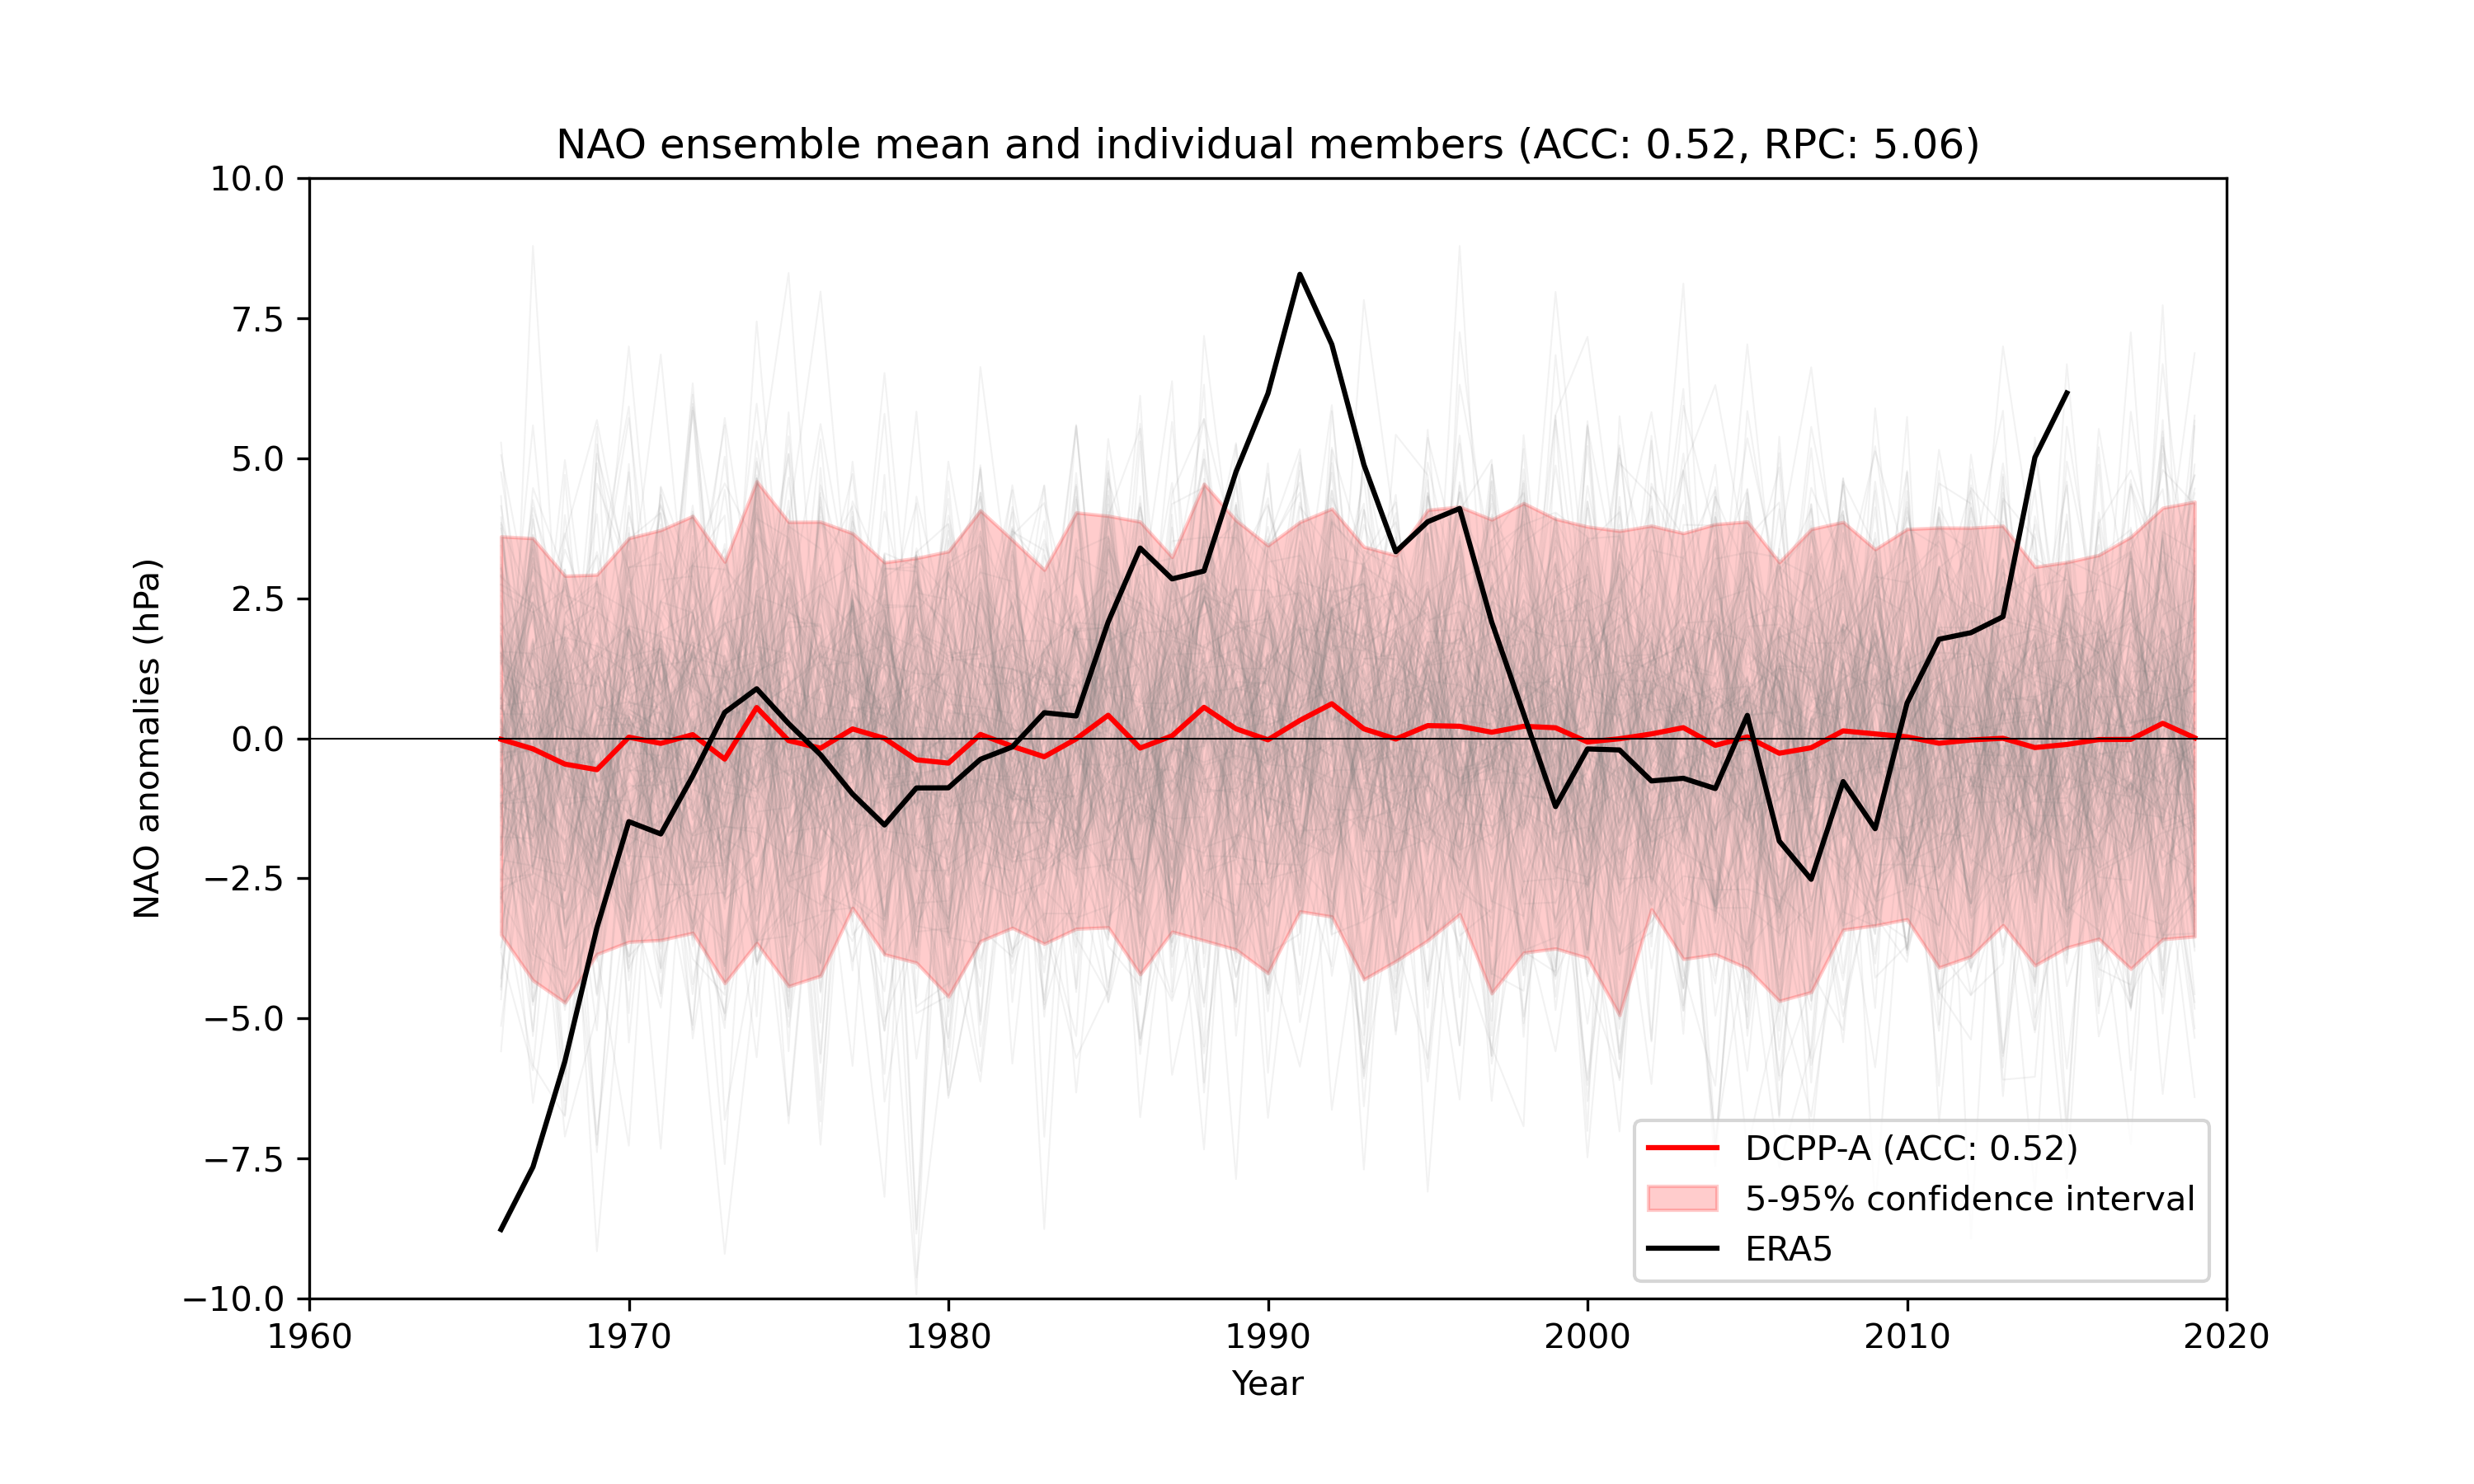
\includegraphics[width=0.45\textwidth]{plots/nao_ensemble_mean_and_individual_members.png}}
    \subfigure[Variance-adjusted and lagged]{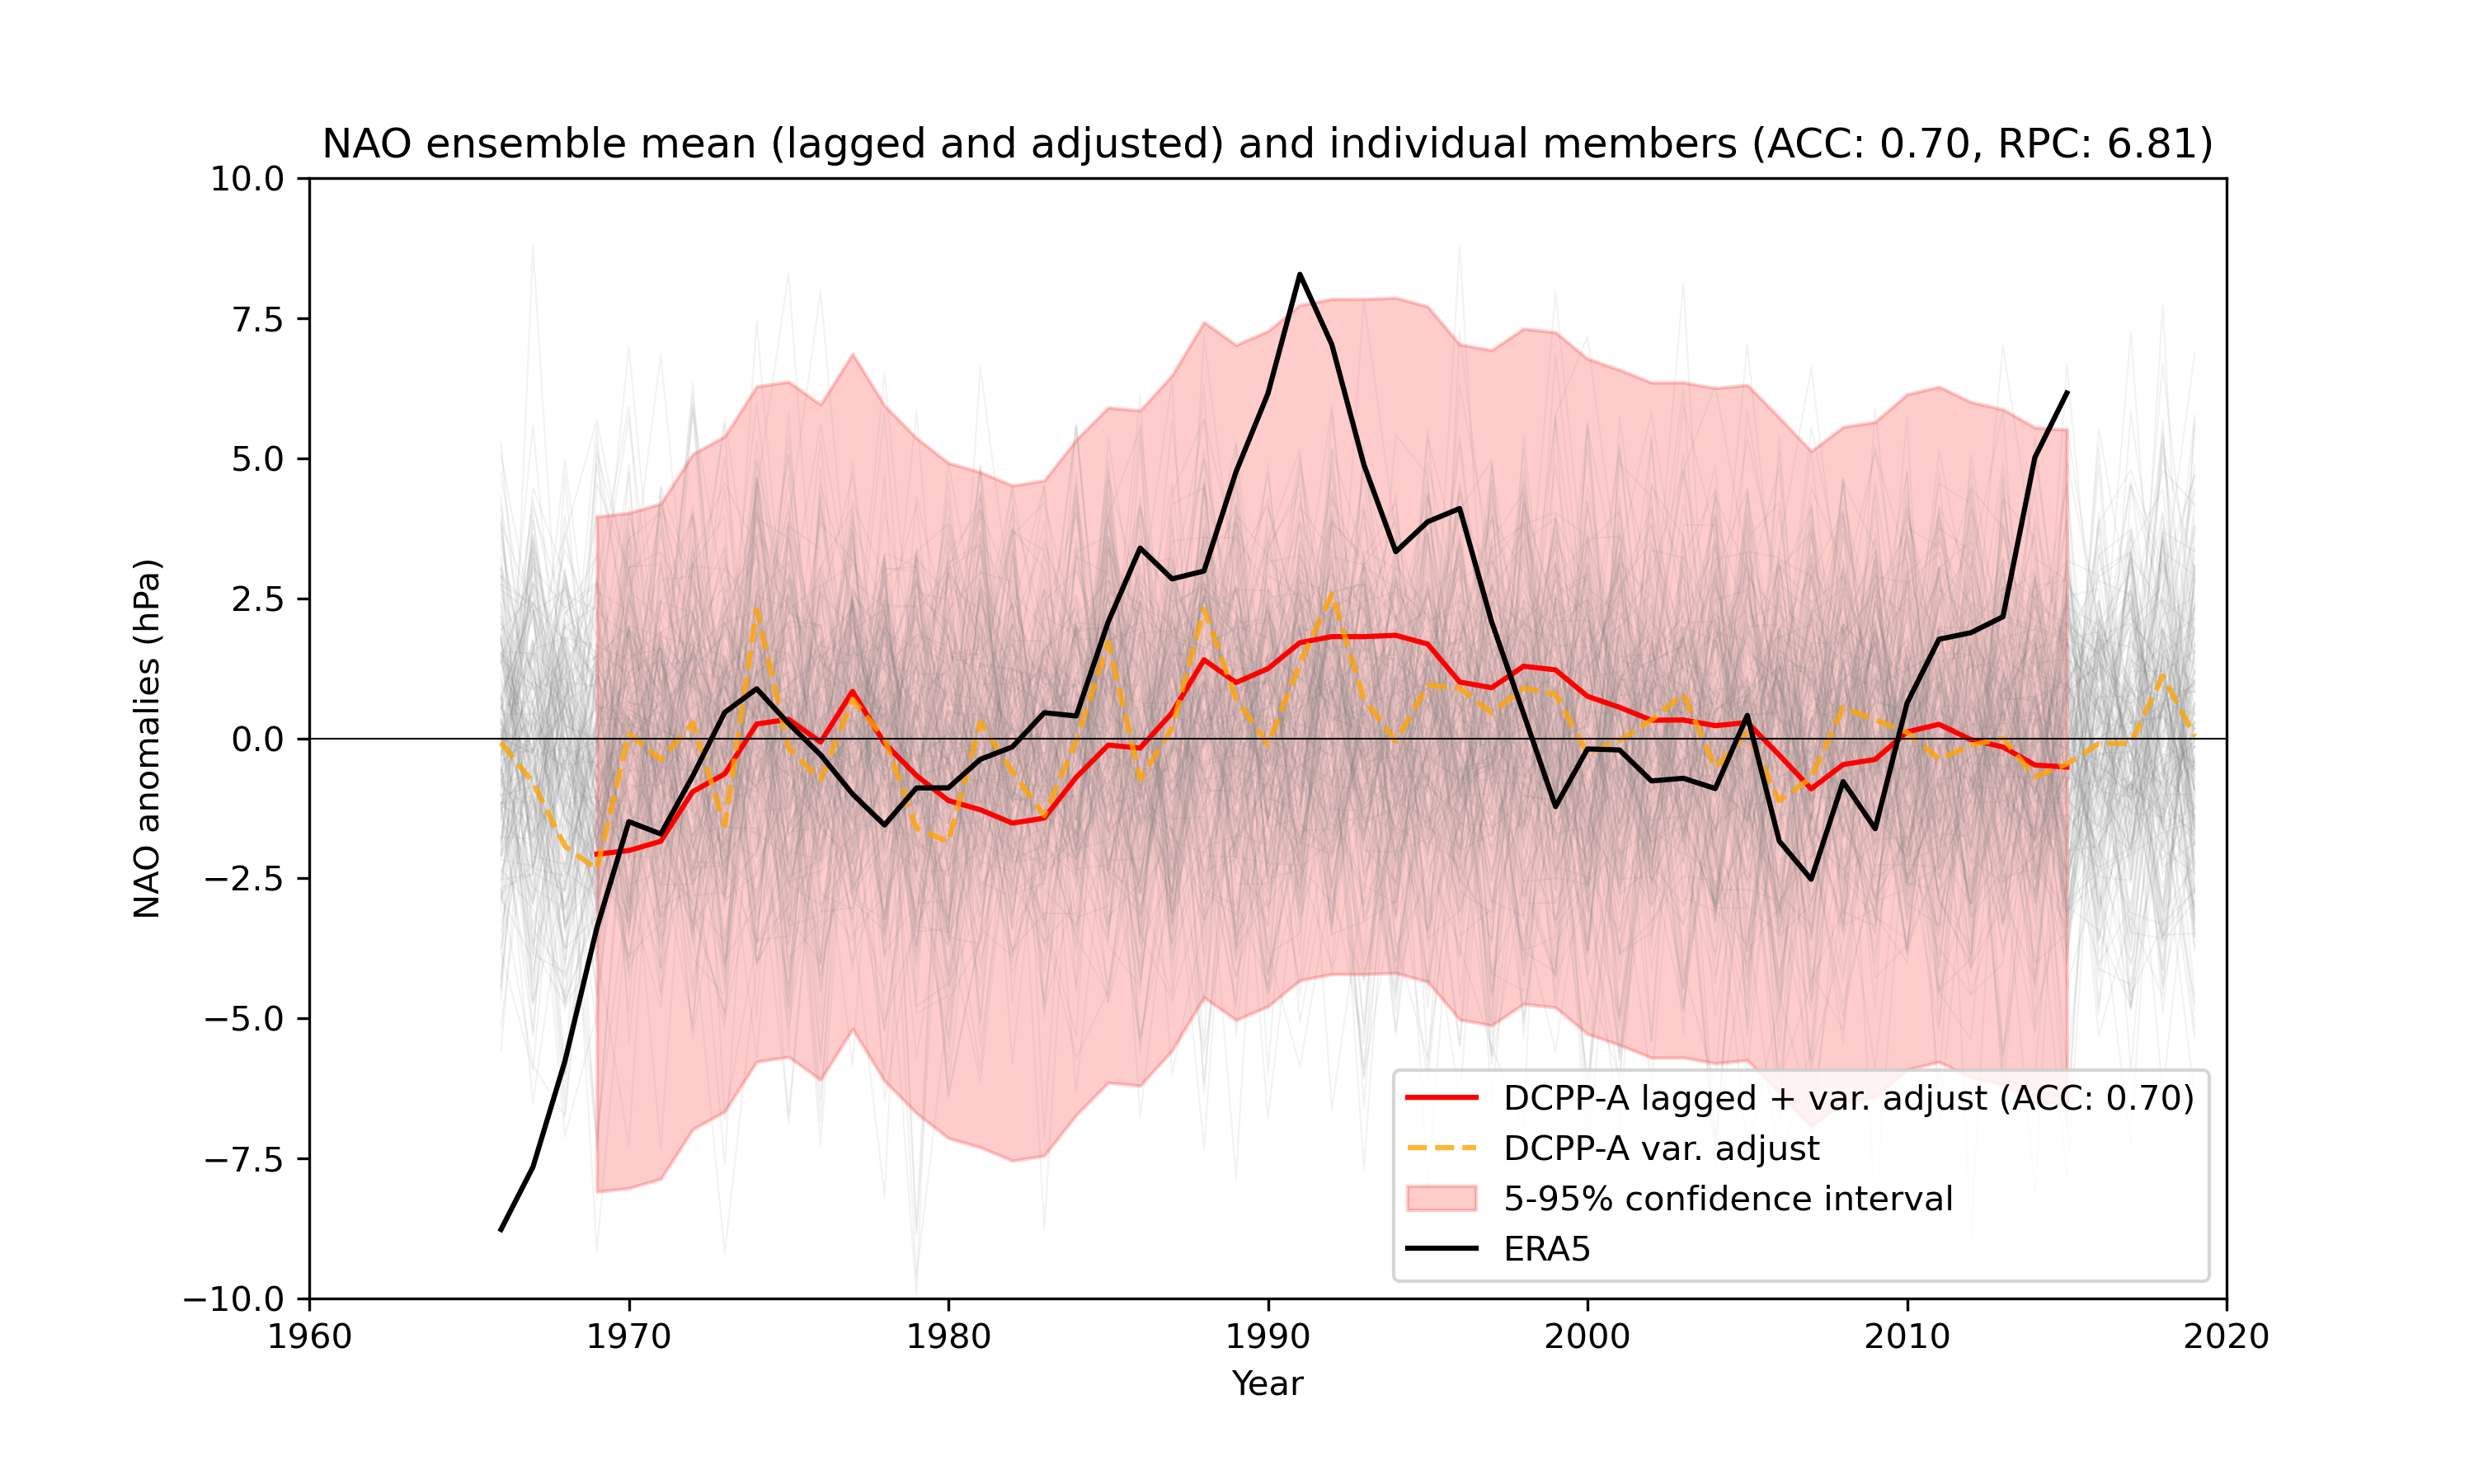
\includegraphics[width=0.45\textwidth]{plots/nao_ensemble_mean_and_individual_members_lagged_and_adjusted.png}}
    \caption{ a. Observed (black) and model-forecast (years 2-9; red) 8-year running means for the boreal winter (DJFM) NAO index. Red curve shows the equally-weighted ensemble mean of all 178 ensemble members. The thin grey lines show the output of each individual ensemble member. The red shading shows the 5\%-95\% confidence interval of all the ensemble members. The anomalies are calculated relative to the average of all year 2-9 boreal winter hindcasts for each model. Observations derive from ERA5. The ACC of the multi-model ensemble mean (for initialization period: 1961-2005) and the RPC are indicated b. As in a. but for the lagged ensemble mean which combines each hindcast with those from the previous three start dates (giving 712 ensemble members). The variance of the ensemble mean is adjusted by normalising by the standard deviation of the ensemble mean. The dashed yellow line shows the variance-adjusted ensemble mean, without lagging. The 5\%-95\% confidence interval is shown by the red shading and is diagnosed from the RMSE between the variance-adjusted ensemble members and the observations.}
    \label{fig:multi-model-means}
\end{figure}

% p values for this
Figure \ref{fig:multi-model-means} shows the observed and model-forecast NAO index for the years 2-9 of the hindcasts. The observations show the decadal variability of the NAO, with a peak in positive NAO conditions around 1990 and a return to these conditions following 2010. While much of the variability is captured by individual ensemble members (thin grey lines), some of the extremes (late 1960, 1990, mid-2010s) aren't captured by the models in figure \ref*{fig:multi-model-means}a. The multi-model ensemble means for the raw ensemble show little predictable signal. Despite this, the models do show skill when predicting the phase of the variability, with significant correlation skill of the ensemble mean (ACC=0.52, P=???) with the observations. This result is comparable with those from \cite{smith2020north}, with ACC=0.48, P=0.03 and \cite{marcheggiani2023decadal} with ACC=0.55, P<0.01. This indicates that skilful model predictions of the NAO are possible, but are comprimised by the low signal-to-noise ratio (RPC=5.06). Therefore the variance must be calibrated to provide realistic, skilful forecasts. 


\section*{Future Work}

\subsection{Short-term}

\subsection{Long-term}

% section detailing the repos in which my scripts are stored
\subsection*{Code Availability}

% print the references
\printbibliography

\section*{Appendix}

The models used, and their ensemble sizes are outlined in table \ref{tab:models}.


% might want to tidy this up slightly
% e.g. with full modelling center names
% and references for each model
\begin{table}[ht]
    \centering
    \caption{Model Information}
    \begin{tabular}{lll}
        \toprule
        Model group & Model & Total ens. members \\
        \midrule
        NCC & NorCPM1 & 20 \\
        NCAR & CESM1-1-CAM5-CMIP5 & 40 \\
        IPSL & IPSL-CM6A-LR & 10 \\
        MIROC & MIROC6 & 10 \\
        CAS & FGOALS-f3-L & 9 \\
        MPI-M/DWD & MPI-ESM1-2-LR & 16 \\
        BCC & BCC-CSM2-MR & 8 \\
        MPI-M & MPI-ESM1-2-HR & 10 \\
        CCCma & CanESM5 & 20 \\
        CMCC & CMCC-CM2-SR5 & 10 \\
        EC-Earth-Consortium & EC-Earth3 & 15 \\
        MOHC & HadGEM3-GC31-MM & 10 \\
        \bottomrule
    \end{tabular}
    % create a label for this table
    \label{tab:models}
\end{table}


% end the file
\end{document}

